\subsection[Reconhecimento]{Reconhecimento}
\begin{frame}
\frametitle{Reconhecimento}

\begin{figure}[H]
\centering
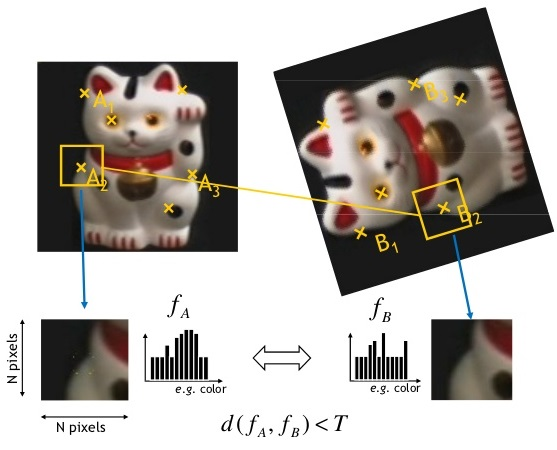
\includegraphics[scale=0.4]{images/reconhecimento}
\caption{Ilustra��o do procedimento de reconhecimento com caracter�sticas
locais.
Fonte \cite{localfeaturedetector}}
\label{fig:reconhecimento}
\end{figure}

\end{frame}

\begin{frame}
Processo de reconhecimento como ilustrado na
imagem~\ref{fig:reconhecimento}:
\begin{itemize}
	\item Encontrar um grupo de \emph{keypoints} distintos;
	\item Definir uma regi�o em torno de cada \emph{keypoint};
	\item Extrair e normalizar o conte�do da regi�o;
	\item Calcular um descritor para a regi�o normalizada;
	\item Encontrar correspond�ncias de descritores.  
\end{itemize}



\end{frame}